% !TEX root = ../../../Masterthesis.tex
\section{Main Title}
\begin{figure}[h!]
\center
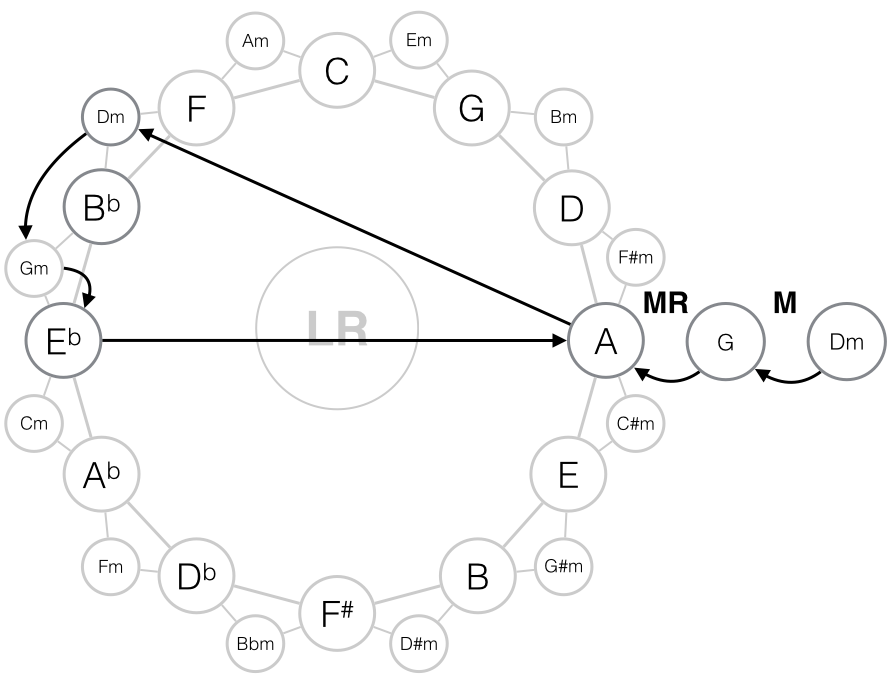
\includegraphics[width=\linewidth]{ST11_main_title}
	\caption{ST 11: Main Title}
	\label{ST_11_main_title}
	\setfloatalignment{b}
\end{figure}
After the action packed encounter with the time traveling Romulans has subsided, the wife of Kirk Senior gives birth to James T. Kirk. The  rhythmical motif of Star Trek begins playing while a fluttering flute plays a melody based upon harmonic minor. In essence, this cue is the same as the first. The motifs are the same with the exception of their order; first comes the rhythmical motif, then the main theme is re-harmonized slightly with \(i-v\) instead of \(i-\flat{VI}\) and, instead of triplets, the theme is stretched out to quarter-notes. 

%-----------------------------------------------------------------------------
% PDF
%-----------------------------------------------------------------------------
\clearpage
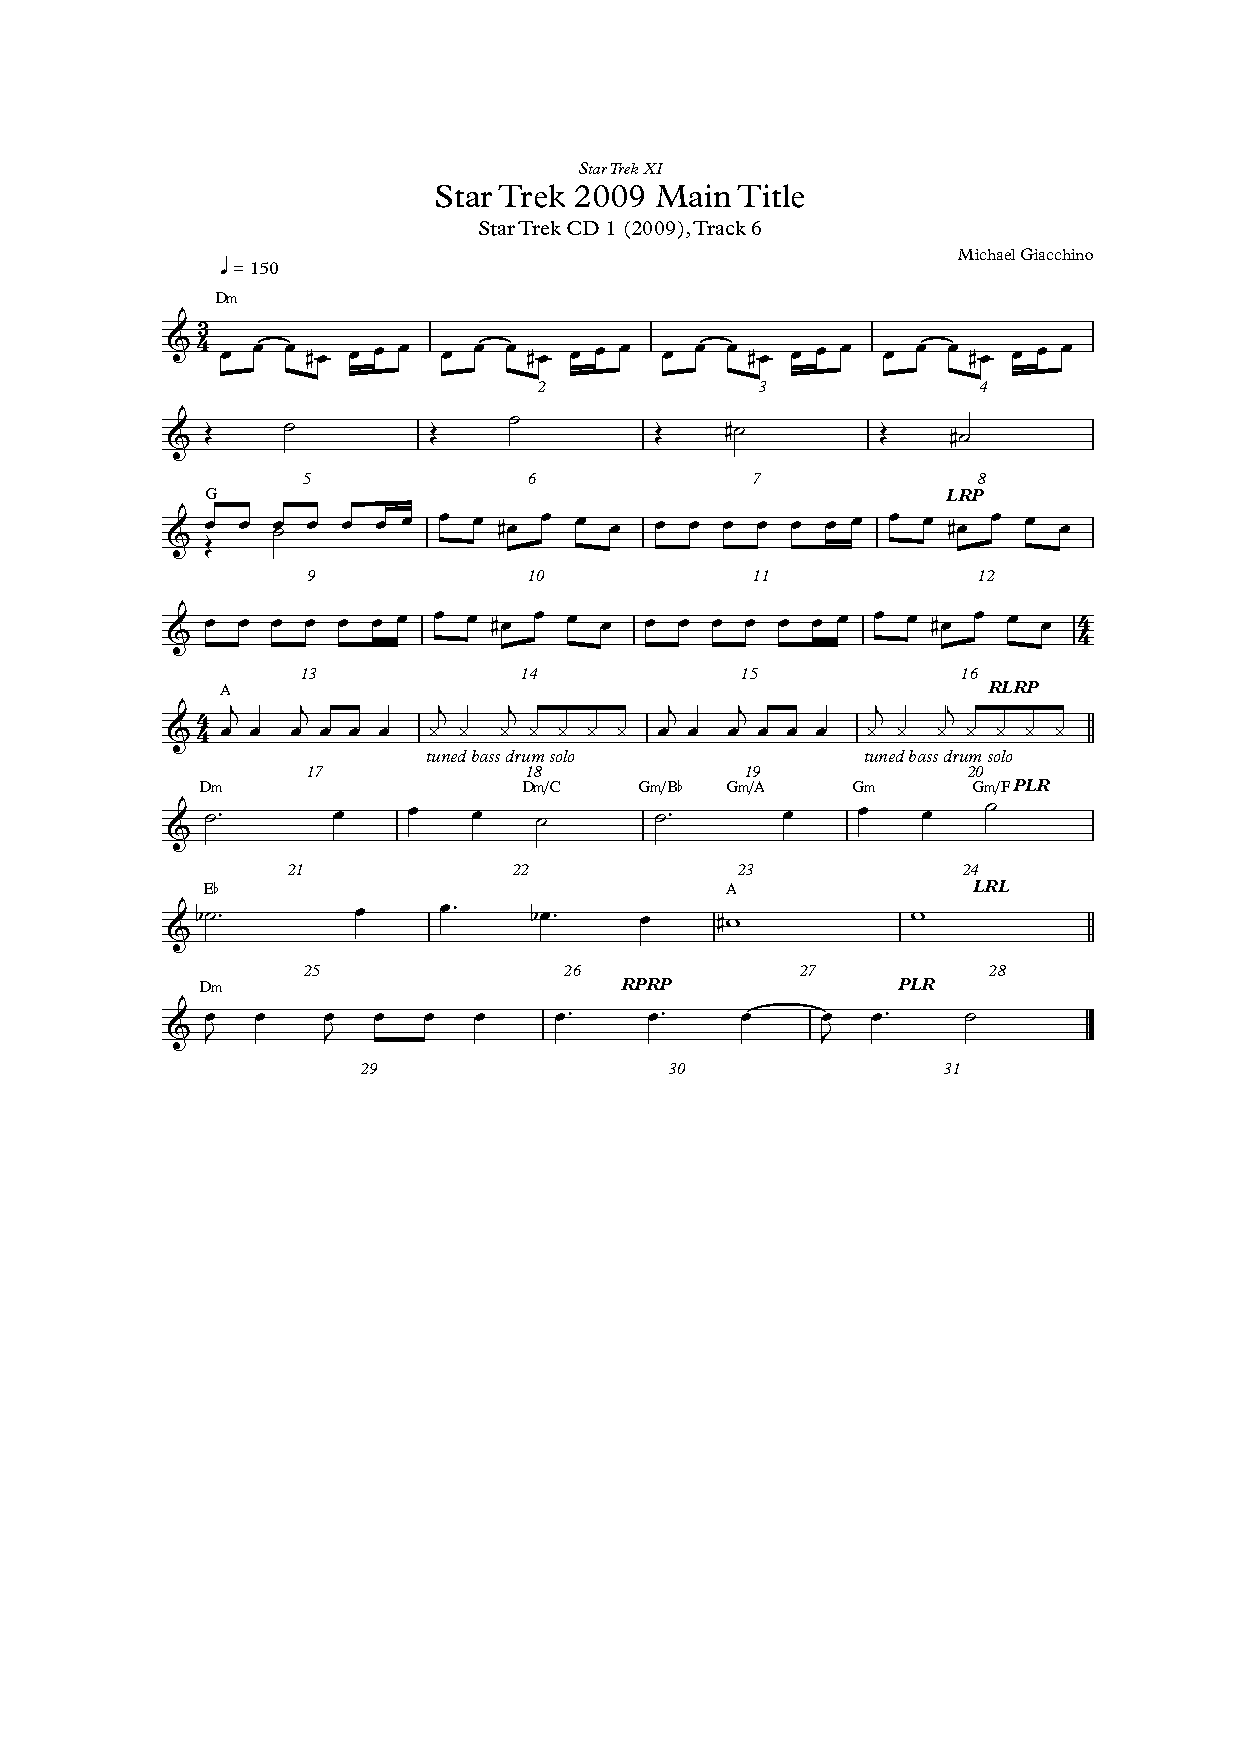
\includepdf[pages=-,pagecommand=\thispagestyle{fancy}]{pdf/ST11/ST_11_2_Main_Title.pdf}

% Reviewed
